\documentclass{beamer}
\title{Wegfindung im Labyrinth (AP)}
\author{\texorpdfstring{Florian Nowak \& Yichuan Shen\\ Betreuer: Gero Plettenberg, Thomas Kloepfer}{Florian Nowak \& Yichuan Shen}}
\date{Wintersemester 2014/15}

%\usetheme{Goettingen}
\setbeamertemplate{navigation symbols}{}

\usepackage[utf8]{inputenc}

\usepackage[ngerman]{babel}
\usepackage{lmodern}
\usepackage{graphicx}
  \graphicspath{{bilder/}}
\usepackage{tikz}
  \usetikzlibrary{shapes}
\usepackage{xparse}
  \NewDocumentCommand\blocking{m}{\textcolor{green}{\textit{#1}}}
  \NewDocumentCommand\blue{m}{{%
  	\usebeamercolor[fg]{frametitle}{#1}%
  }}
\usepackage[default]{sourcesanspro}
%\usepackage[default,osfigures,scale=0.9]{opensans}

\begin{document}
\maketitle

\begin{frame}[fragile,t]{Aufgabenstellung}
Ein bereits vorhandener Roboter mit neigbarem Touchscreen soll etwas Neues lernen: Er soll ein beliebiges auf dem Rahmen seines Touchscreens aufliegendes Labyrinth (vorgegebener Rastergröße) mithilfe einer Metallkugel einlesen können. Der Roboter kann eine solche Kugel bereits auf eine ihm vorgegebene Position durch Kippen rollen lassen (und dort auch zum Stillstehen bringen). Das Ziel ist es somit, den Roboter ein zuvor eingelesenes Labyrinth mit der Kugel (auf optimalem Weg) lösen zu lassen.

\medskip\noindent
\blocking{Aufgabenstellung am Roboter erläutern!}
\end{frame}

\begin{frame}[fragile,t]{Vorstellung}
\blocking{Kurz vorstellen!}
\end{frame}

\begin{frame}[fragile,t]{Demonstration}
\blocking{\verb~string~-Darstellung des vorhandenen Labyrinths einlesen und Labyrinth lösen! Anschließend mit der Tiefensuche beginnen!}
\end{frame}

\begin{frame}[fragile,t]{Praktikumsverlauf}
\begin{enumerate}
 \item \blue{Einarbeitung} \textit{(bis Anfang Dezember)}\blue{:} Vorgängercode und Funktionsfähigkeit des Roboters testen.
 \item \blue{Durchlaufen des Labyrinths} \textit{(bis Anfang Januar)}\blue{:}\\
 Durch Vorgabe eines Labyrinths als Datenstruktur soll die Kugel einen beliebig vorgegebenen Pfad durchlaufen können. Ferner wird ein optimaler Weg durch das Labyrinth berechnet.
 \item \blue{Erkennen des Labyrinths} \textit{(bis Ende Januar)}\blue{:}\\
 Durch Ablaufen eines realen Labyrinths soll die Struktur des Labyrinths erkannt und abgespeichert werden. Dafür wird ein Algorithmus entworfen und implementiert.
 \textcolor{gray}{
 \item[\textcolor{gray}{4.}] Fertigstellung \textit{(bis Anfang März)}:\\
Präsentation, Poster und Webseite fertig stellen; ggf. eine grafische Oberfläche erstellen.
}
\end{enumerate}
\end{frame}

\begin{frame}[fragile,t]{Praktikumsverlauf}
Unseren Zeitplan konnten wir recht gut einhalten. Der dritte Milestone ist wie erwartet aufwendiger geworden, erreicht haben wir ihn erst nach den Klausuren (also Mitte Februar). Hinzugekommen sind optische Verbesserungen an der Hardware. \blocking{Letztere am Roboter zeigen!}

\smallskip
\begin{enumerate}
 \item[3.] \blue{Erkennen des Labyrinths (Tiefensuche)}
 \begin{enumerate}
 \item[(a)] Entwurf einer Routine zur Wanderkennung
 \item[(b)] Optimierung (hinsichtlich Geschwindigkeit)
 \end{enumerate}
 \item[\textcolor{gray}{4.}] \textcolor{gray}{Fertigstellung}
\end{enumerate}
\end{frame}

\begin{frame}[fragile,t]{Herangehensweise an die Problemstellung}
\begin{itemize}
\item Festlegung von \blue{Python (2.7)} als Programmiersprache
\item Auswahl des fortan zugrunde liegenden MCU-Codes, Einarbeitung und Reduktion auf die wesentlichen Routinen
\item Erweiterung des Roboter um eine serielle Schnittstelle, Herstellung der Kommunikation zwischen Computer und MCU
\begin{itemize}
\item Auslesen der Kugelposition
\item Schicken einer neuen Position
\item Schreiben einer Python-Klasse für den Touchscreen (\verb~Balancer~-Klasse)
\end{itemize}
\item Speicherung des Labyrinths als rechteckiger, einfacher Graph: Schreiben der \verb~Maze~-Klasse
\end{itemize}
\blue{Code-Aufteilung:}
\begin{figure}[h]
  \centering
  \begin{tikzpicture}[
    text centered,
	rounded/.style={
	  rounded rectangle,
	  very thick,
	  draw=lime!50!black!70,
	  top color=white,
	  bottom color=lime!50!black!30
	},
	block/.style={
	  rectangle,
	  very thick,
	  draw=black!50,
	  top color=white,
	  bottom color=black!20
	},
 	line/.style={draw, thick}
	]
	\node [block] at (0, 0) (main) {\verb~main.py~};
	\node [rounded] at (-3, 0) (maze) {\verb~Maze~};
	\node [rounded] at (3, 0) (balancer) {\verb~Balancer~};
	\node [block, dashed] at (0, 1) (mcu) {MCU-Code};
	\node at (-3, 1) (labyrinth) {Labyrinth};
	\node at (3, 1) (touchscreen) {Touchscreen};
	\path[line] (main) -- (balancer);
	\path[line, dashed] (balancer) -- (mcu);
	\path[line] (main) -- (maze);
	\draw[line, <->] (maze) -- (labyrinth);
	\draw[line, <->] (balancer) -- (touchscreen);
  \end{tikzpicture}
\end{figure}
\end{frame}

\begin{frame}[fragile,t]{Ergebnis}
\begin{figure}
  \centering
  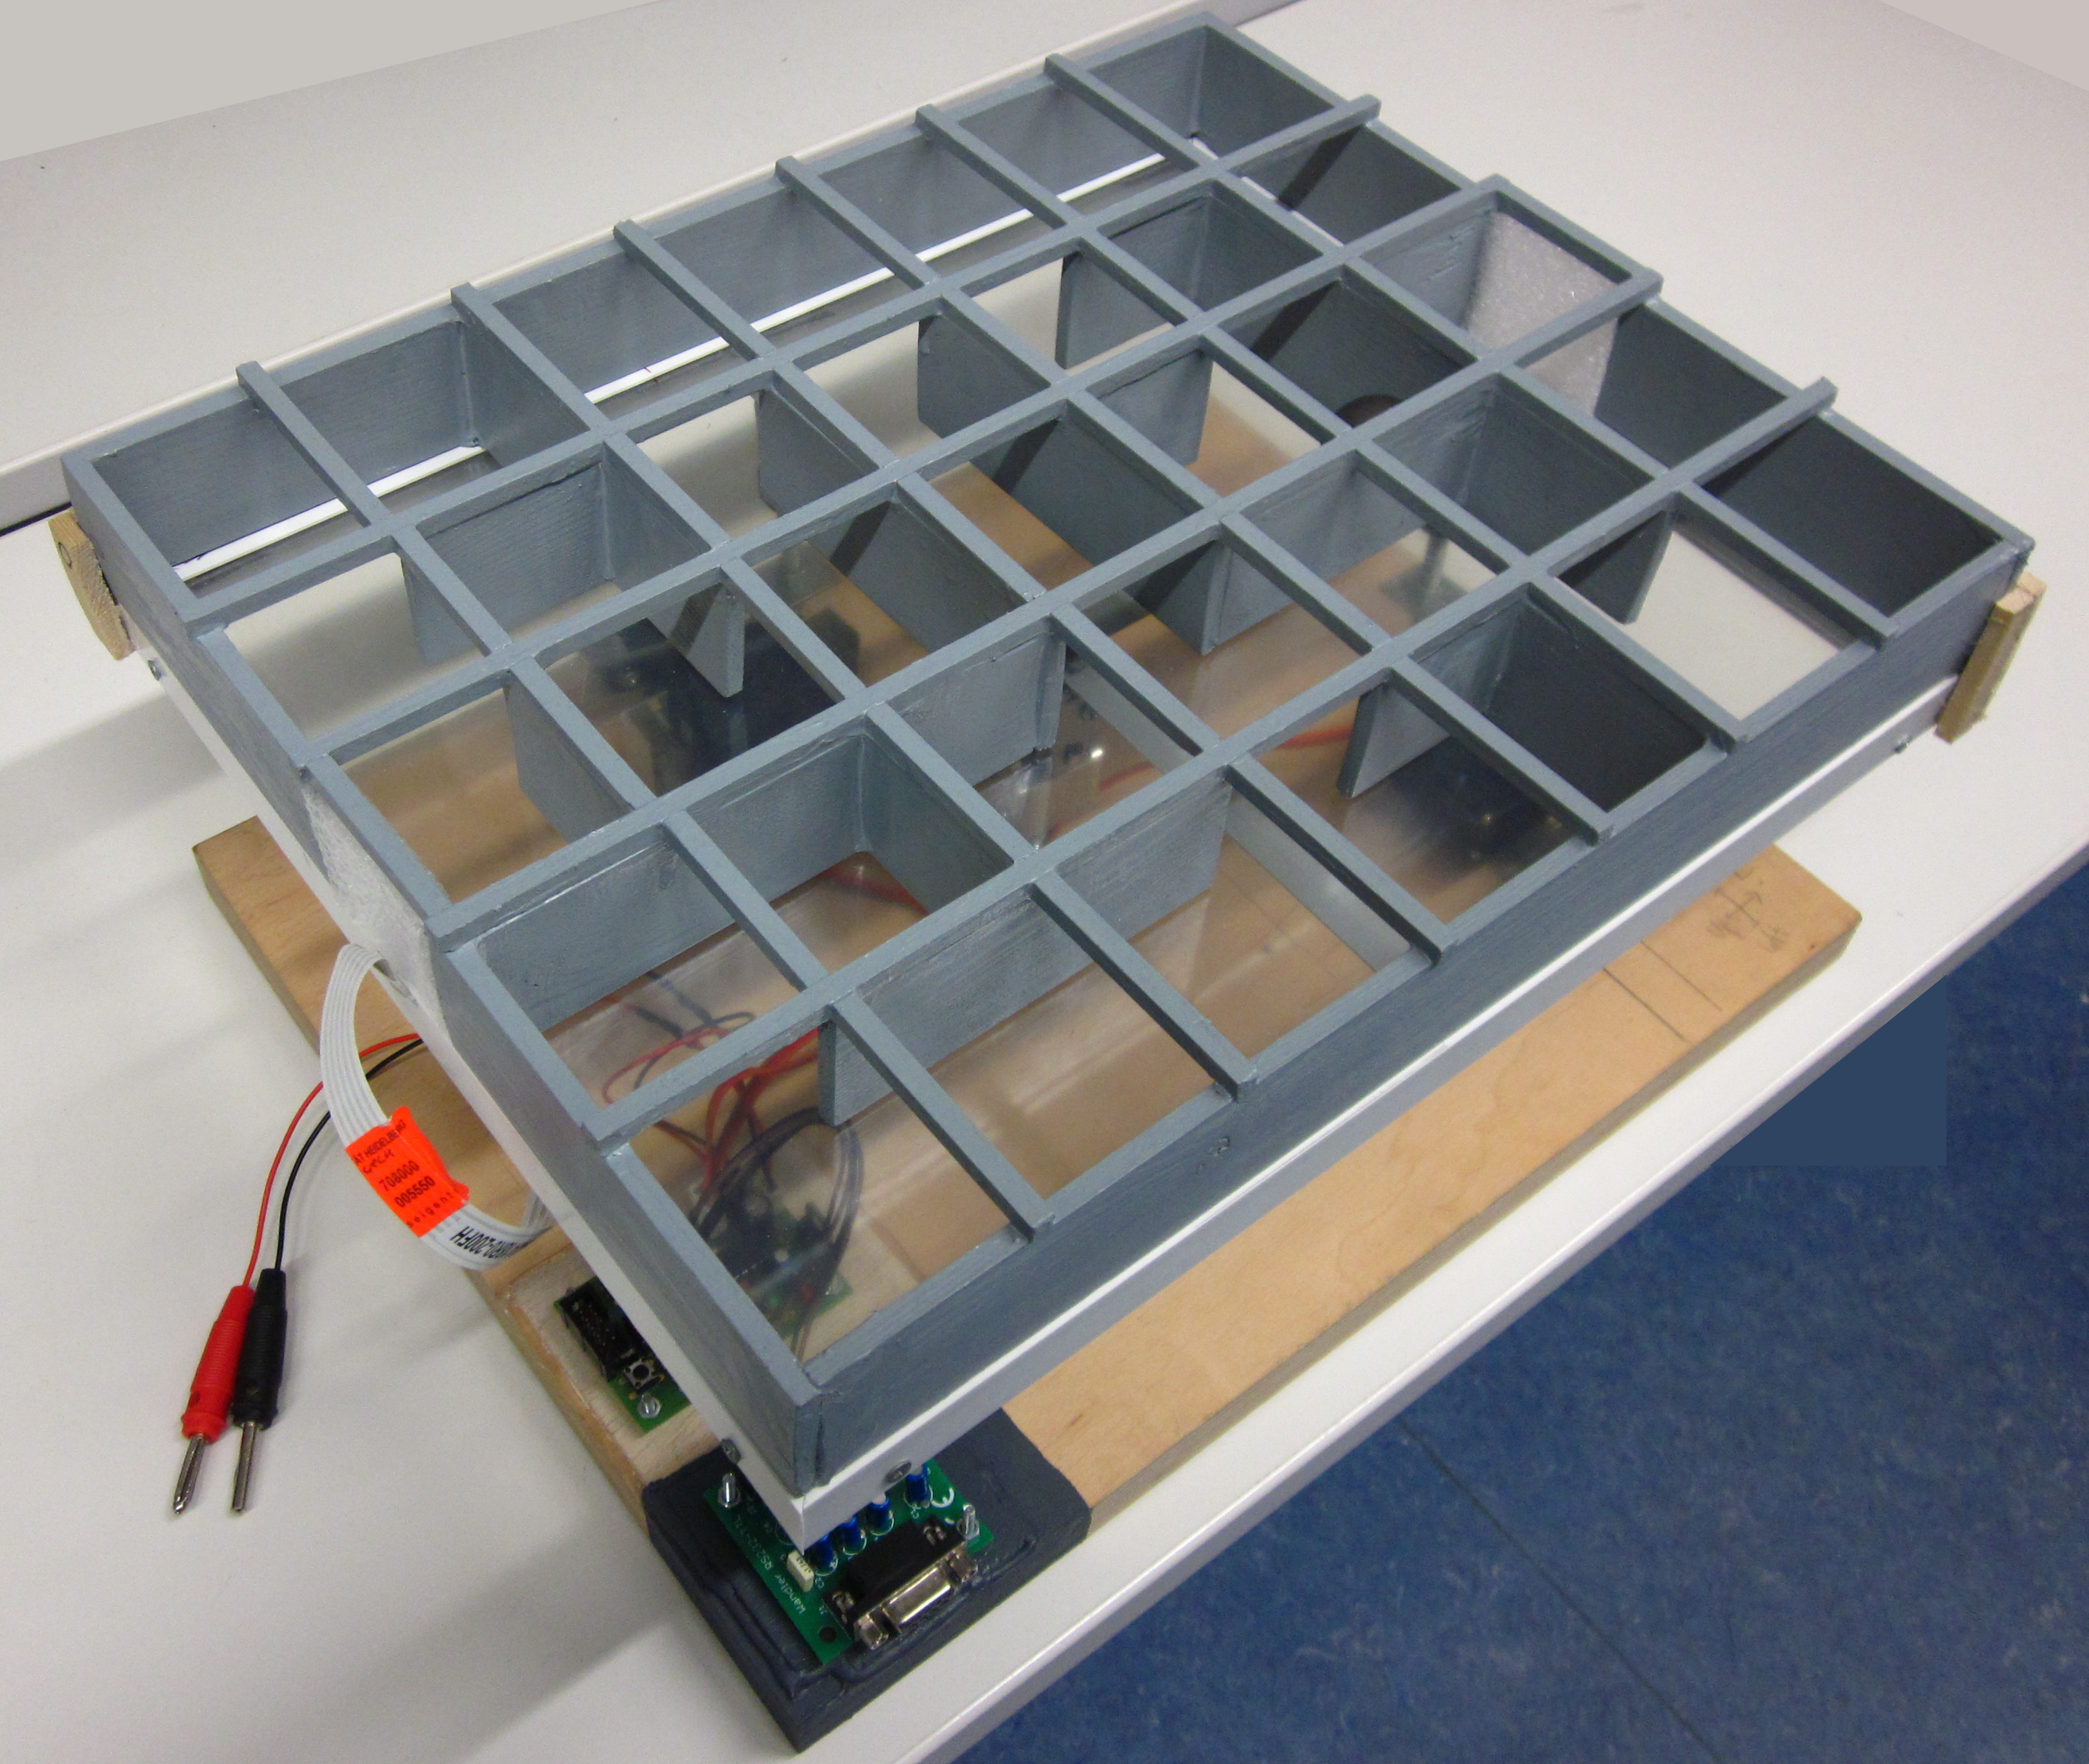
\includegraphics[scale=.2]{roboter_badly-photoshoped}
  %\caption{}
\end{figure}
\end{frame}

\begin{frame}[fragile,t]{Die \verb~Maze~-Klasse}
Text.
\end{frame}

\begin{frame}[fragile,t]{Die \verb~Balancer~-Klasse}{Kommunikation zwischen PC und MCU}
Text.
\end{frame}

\begin{frame}[fragile,t]{Ablauf der Wanderkennung}
\begin{small}
\begin{figure}[h]
  \centering
  \begin{tikzpicture}[
    text centered,
	rounded/.style={
	  rounded rectangle,
	  text width=1cm,
	  very thick,
	  draw=red!50!black!70,
	  top color=white,
	  bottom color=red!50!black!30
	},
	kugel/.style={
	  rounded rectangle,
	  text width=2.5cm,
	  very thick,
	  draw=blue!50!black!70,
	  top color=white,
	  bottom color=blue!50!black!30
	},
	block/.style={
	  rectangle,
	  text width=3cm,
	  very thick,
	  draw=black!50,
	  top color=white,
	  bottom color=black!20
	},
 	line/.style={draw, thick, ->}
	]
	\node at (0, 0) [rounded] (start) {Start};
	\node at (0, -1.5) [block] (nstack) {Generiere \verb~neighbors_stack~ von \verb~anchor~};
	\node at (0, -3.5) [block] (init) {Initialisierung: Balanciere Kugel auf \verb~anchor~ aus};
	\node at (0, -5.3) [kugel] (kugel) {Kugel ist ausbalanciert};
	\path [line] (start) -- (nstack);
	\path [line] (nstack) -- (init);
	\path [line] (init) -- (kugel);
  \end{tikzpicture}
\end{figure}
\end{small}
\end{frame}

\begin{frame}[fragile,t]{Ablauf der Wanderkennung}
\begin{tiny}
\begin{figure}[h]
  \centering
  \begin{tikzpicture}[
    text centered,
	rounded/.style={
	  rounded rectangle,
	  text width=.7cm,
	  very thick,
	  draw=red!50!black!70,
	  top color=white,
	  bottom color=red!50!black!30
	},
	kugel/.style={
	  rounded rectangle,
	  text width=1.25cm,
	  very thick,
	  draw=blue!50!black!70,
	  top color=white,
	  bottom color=blue!50!black!30
	},
	block/.style={
	  rectangle,
	  text width=1.75cm,
	  very thick,
	  draw=black!50,
	  top color=white,
	  bottom color=black!20
	},
	decision/.style={
	  diamond,
	  text width=1cm,
	  very thick,
	  draw=lime!50!black!70,
	  top color=white,
	  bottom color=lime!50!black!30
	},
 	line/.style={draw, thick, ->}
	]
	\path[draw, thick, dashed, blue!50!black!70] (0, -6) -- (0, -6.5) -- (-1.125, -6.5) -- (-1.125, 0) -- (0, 0);
    \node at (0, 0) [kugel] (kugelstart) {Kugel ist ausbalanciert};
	\node at (-2, 0) [rounded] (ende) {Ende};
	\node at (2, 0) [block, text width=1cm] (nochmal) {Versuche es erneut};
	\node at (0, -1.5) [decision] (ziel) {Ist die Kugel am Ziel?};
	\node at (-3, -1.5) [decision, text width=1.675cm] (leer) {Ist \verb~neighbors_stack~ leer?};
	\node at (3, -1.5) [decision] (anker) {Ist \verb~anchor~ das Ziel?};
	\node at (0, -4) [block, text width=1cm] (erreichbar) {$n$ ist erreichbar};
	\node at (-3, -4) [decision] (nachbar) {Ist Ziel ein Nachbar $n$?};
	\node at (3, -4) [decision] (versucht) {Bereits zweimal versucht?};
	\node at (0, -5) [block, text width=1cm] (zurueck) {Gehe zurück zu \verb~anchor~};
	\node at (-4, -6) [block, text width=2cm] (weiter) {Hole einen (neuen) Nachbarn $n$ aus \verb~neighbors_stack~ und schicke die Kugel dorthin};
	\node at (4, -6) [block, text width=1.25cm] (wand) {Zwischen \verb~anchor~ und $n$ ist eine Wand};	
	\node at (0, -6) [kugel] (kugelende) {Kugel ist ausbalanciert};
	\node at (2, -6) [block, text width=1.375cm] (servos) {Setze die Servomotoren zurück};
	\path[line] (nochmal) -- (kugelstart);
	\path[line] (leer) -- node [left] {J} (ende);
	\path[line] (kugelstart) -- (ziel);
	\path[line] (anker) -- node [right] {J} (nochmal);
	\path[line] (ziel) -- node [above] {J} (leer);
	\path[line] (ziel) -- node [above] {N} (anker);
	\path[line] (leer) -- node [left] {N} (nachbar);
	\path[line] (anker) -- node [right] {N} (versucht);
	\path[line] (nachbar) -- node [above] {J} (erreichbar);	
	\path[line] (nachbar) -- node [left] {N} (weiter);
	\path[line] (erreichbar) -- (zurueck);
	\path[line] (versucht) -- node [right] {J} (wand);
	\path[line] (4, -4) -- node [right] {N} (4, 0) -- (nochmal);
	\path[line] (weiter) -- (kugelende);
	\path[line] (zurueck) -- (kugelende);
	\path[line] (wand) -- (servos);
	\path[line] (servos) -- (kugelende);
  \end{tikzpicture}
\end{figure}
\end{tiny}
\end{frame}

\begin{frame}[fragile,t]{Optimierung}
\begin{itemize}
\item Die Funktion \verb~run(path, maze)~ berücksichtigt durch \verb~maze.get_skippables(path)~ erhaltene Felder
\item \verb~detect_walls~ lässt die Kugel auf dem letzten Nachbarn, falls dieser erreichbar war
\item \verb~detect_maze~ berücksichtigt die Ausgabe von \verb~detect_walls~ und verhindert unnötige Wege
\end{itemize}
\end{frame}

\begin{frame}[fragile,t]{Aufgetretene Probleme}
Durch den unempfindlichen inneren Rand des Touchscreens dauert das Ausbalancieren in Randnähe durchschnittlich länger. Auch in verhältnismäig kleinen Labyrinthfeldern können Verzögerungen bei der Erkennung des Labyrinths auftreten. Die naheliegende Lösung beider Probleme ist eine Verbesserung der Hardware.
\end{frame}

\begin{frame}[fragile,t]{Ausblick/Reflektion}
Das Praktikum hat uns sehr gefallen und war ein guter Ausgleich zu unseren Vorlesungen.

\medskip\noindent
Wir denken nicht, dass sich der Roboter (bezogen auf unsere Aufgabenstellung) wesentlich verbessern lässt. Mögliche Erweiterungen:
\begin{itemize}
\item Labyrinthmaße experimentell bestimmen lassen
\item GUI schreiben
\textcolor{gray}{
\item[\textcolor{gray}{$\triangleright$}] Hardware erneuern und optimieren (beinhaltet Arbeit am MCU-Code)
}
\end{itemize}
\end{frame}


%\begin{frame}[fragile,t]{Thema}{Unterthema}
%\verb~print('Hello world!')~
%\end{frame}

\end{document}
